\subsection{Efficiency}
	We performed the numerical simulation of 
	\begin{equation}
		dy(t) =  -y^5 dt + ydw(t), \qquad y(0) = 1.
	\end{equation}
	\begin{figure}
		\centering
		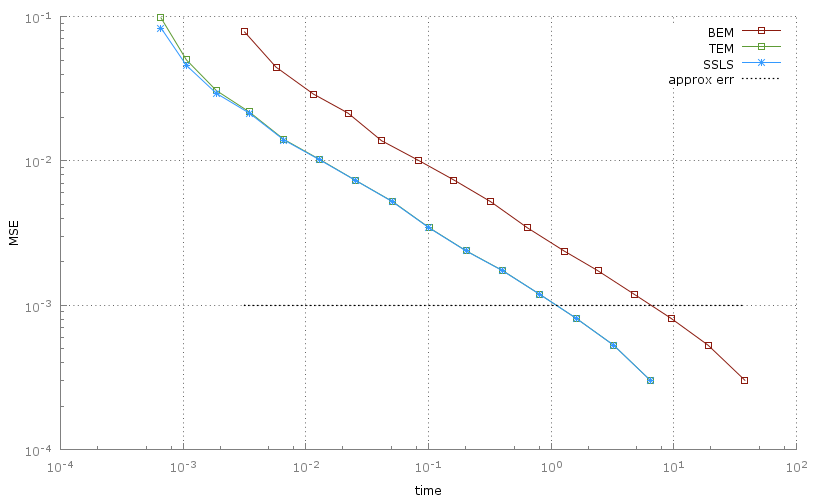
\includegraphics[width=0.7\linewidth]{./papers/paperB/figures/MSETime2}
		\caption{}
		\label{fig:MSETime2}
	\end{figure}
\subsection{Positivity of solutions}
First we consider the Lotka Volterra equation \cite{Mao2007a}
\begin{equation}\label{eqn:LotkaVolterra}
	dy(t)= \left[by(t)-a y(t)^2\right]dt + \sigma y(t) dW_t,
\end{equation}
which have exact solution
\begin{equation}\label{eqn:LotkaVolterraSol}
	y(t) = \frac{
		y_0
		\exp\left[
		b-\frac{1}{2}\sigma^2) t
		+\sigma W_t
		\right]
		}{
		\displaystyle
		1+a 
		y_0
		\int_0^t
		\exp\left[
		(b -\frac{1}{2})s
		+\sigma W_s
		\right]ds
	}.
\end{equation}
\begin{figure}
	\centering
	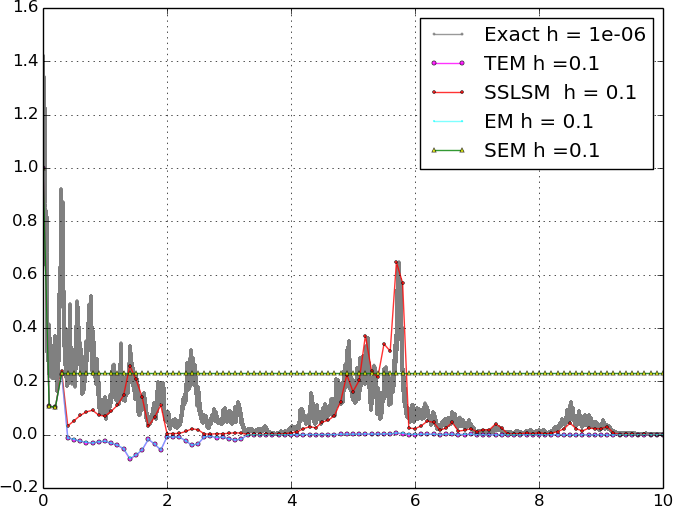
\includegraphics[width=0.7\linewidth]{./papers/paperB/figures/PathsLVEv4}
	\caption{}
	\label{fig:PathsLVEv4}
\end{figure}

